\documentclass[letterpaper]{article}
\usepackage[left=1in,right=1in,top=1in,bottom=1in]{geometry}

\title{Outline for MOF energy histogram work}
\author{Ben Bucior, N. Scott Bobbitt, Arun Gopalan, Neda Bagheri, Randy Snurr}

\usepackage[hidelinks]{hyperref}
\usepackage{graphicx}
\usepackage{amsmath}
\usepackage{comment}

\usepackage[section]{placeins}  % Float barrier between sections, per https://tex.stackexchange.com/questions/4854/floats-how-to-restrict-floating-to-subsection-only-in-one-section-of-the-docum

\usepackage{outlines}
\usepackage{hyperref}
\usepackage{chemscheme}

\newcommand{\red}[1]{\textcolor{red}{#1}}

\begin{document}

\maketitle

%\begin{abstract}
%
%\end{abstract}

\section{Notes}
\begin{outline}
	\1 The Guest Editors Andrew Ferguson and Johannes Hachmann for the special issue chaired my session at AIChE.
	\1 Themed issue "Machine Learning and Data Science in Materials Design" for the journal \textit{Molecular Systems Design \& Engineering}
\end{outline}


\section{Title}
\begin{outline}
	\1 (scratch work.  Let's come back to this later.)
	\1 (from AIChE) Identifying New Descriptors for Gas Storage in Nanoporous Materials
\end{outline}

\section{Requirements and future directions}

\subsection{Quick tasks}
\begin{outline}
	\1 Fill in the remainder of the figures I could see for this paper
	\1 Debrief with Scotty and get his input on availability and possible directions for the manuscript.  He might have some good figures we should adapt for the manuscript, too.
	\1 Do we pre-set the upper and/or lower bounds of the histograms?
	\1 Check out the long-tail(?) of the parity plot (top right, below the parity line).  Could be another variable we need to account for
	\1 Need to comment on nonlinearity somewhere, based on question from AIChE session
	\1 What is the original distribution of y?
\end{outline}

\subsection{Potential directions}
\begin{outline}
	\1 \textbf{How general} is the method?  Just hMOFs?  Also ToBaCCo?
		\2 Could retrain on ToBaCCo and compare coefs
		\2 IZA database of zeolites?
		\2 CCDC MOFs - test model on 1000 MOFs, check agreement, then screen the rest of them?
	\1 Identify old sources of \textbf{GCMC data for reuse} (email Diego or others?)
	\1 \textbf{Other gases:} methane, xenon, multi-site molecules?
	\1 \textbf{Experimental collaboration:} Screening the CCDC MOFs to identify top candidates for hydrogen storage (Would likely take a few weeks at best)
	\1 \textbf{Isotherm prediction or Langmuir rationalization:} Repeat the predictions on multiple pressures (possibly temperatures as well).  What do the coefficients look like?  Is it similar to the Langmuir intuition on how much variability there will be?
	\1 \textbf{Temperature dependence/optimization:} Could also consider changing temperature.  Cryo vs. room temperature adsorption?
\end{outline}


\section{Introduction}

\begin{outline}
	\1 Hydrogen storage challenge
	\1 MOFs and MOF databases
	\1 Screening MOFs for hydrogen storage
		\2 Scotty/Jiayi paper
		\2 Yamil, Diego works
	\1 Use of ML in the MOF literature
		\2 APRDF
		\2 Recent work from U Connecticut
		\2 See also my section in the \href{https://www.elsevier.com/books/modelling-and-simulation-in-the-science-of-micro-and-meso-porous-materials/catlow/978-0-12-805057-6}{review book}
		\2 Relation for the Coulomb descriptor and related proxies in the literature (heat of adsorption, etc.)
\end{outline}



\section{Methods}

\subsection{Calculating the energy grid}

\begin{figure}[!ht]
	\centering
	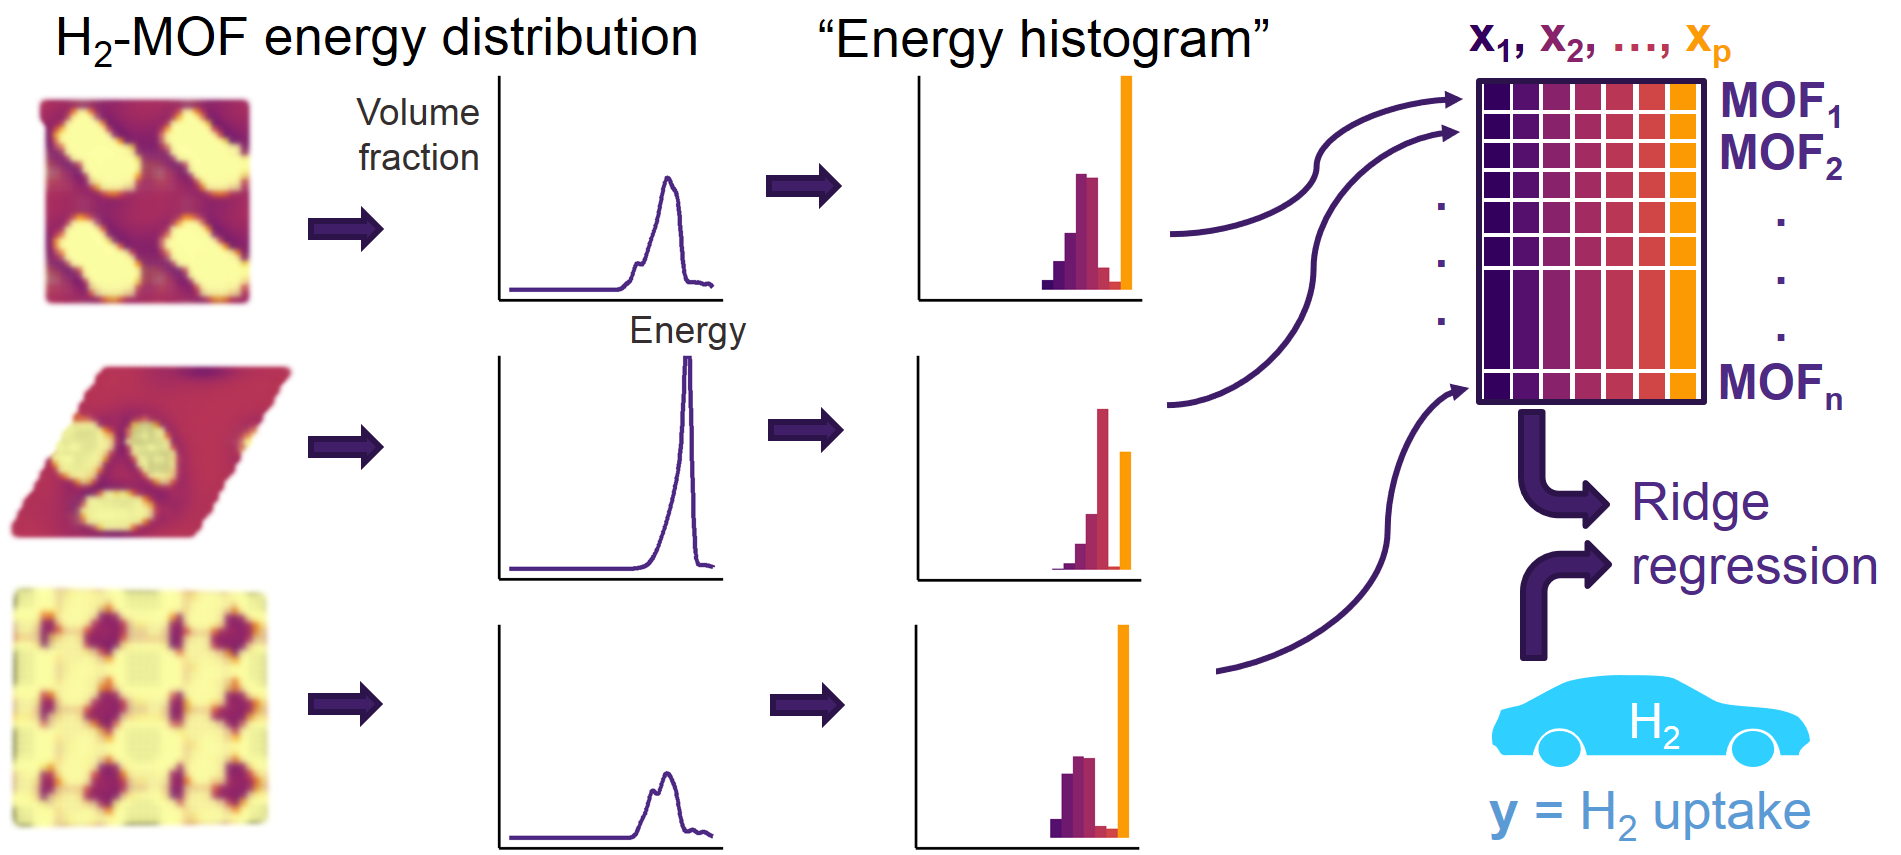
\includegraphics[width=0.75\columnwidth]{Figs/energy_schematic.png}
	\caption{Calculation of the energy histogram from inputs}
	\label{fig:schematic}
\end{figure}


\subsection{Molecular simulations}

\begin{outline}
	\1 RASPA
	\1 Force field parameters for host and guests
	\1 Number of cycles and/or source of data
	\1 Structures
		\2 Wilmer's hMOFs
		\2 Likely ToBaCCo, so we can also look at structural diversity
		\2 Cleaning up the CCDC MOF subset using their solvent removal scripts, etc.
\end{outline}


\subsection{Data processing}

\begin{outline}
	\1 Ridge regression
		\2 Equations and loss function
		\2 R package \verb|glmnet|
			\3 Finding the greatest lambda within 1 SE of the lambda that minimizes model error
	\1 Data preprocessing: z-score bins and remove columns with zero variance.  Also filter out unphysical uptake (< 0 g/L) from GCMC with giant error bars
	\1 Define equations used for model evaluation: Q2, RMSE, MAE
\end{outline}



\section{Results and discussion}

\subsection{LJ metric}
\begin{outline}
	\1 Inspiration from "binding fraction"
	\1 Ask Scotty about this section.  Figures of different distributions?  Comparing MOFs that bind too strongly, etc?
\end{outline}

\subsection{Ridge regression}
\begin{outline}
	\1 Formalizing the results from LJ metric studies
	\1 Meaning of betas and intuition
	\begin{figure}[!ht]
		\centering
		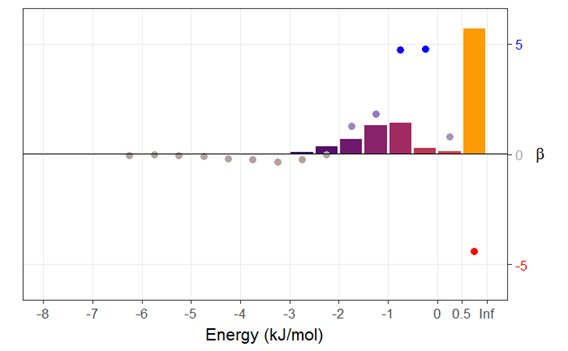
\includegraphics[width=0.75\columnwidth]{Figs/betas.png}
		\caption{Regression coefficients overlaid on the histogram}
		\label{fig:betas}
	\end{figure}
	\1 How good is the model and fit?
		\2 Parity plot
		\begin{figure}[!ht]
			\centering
			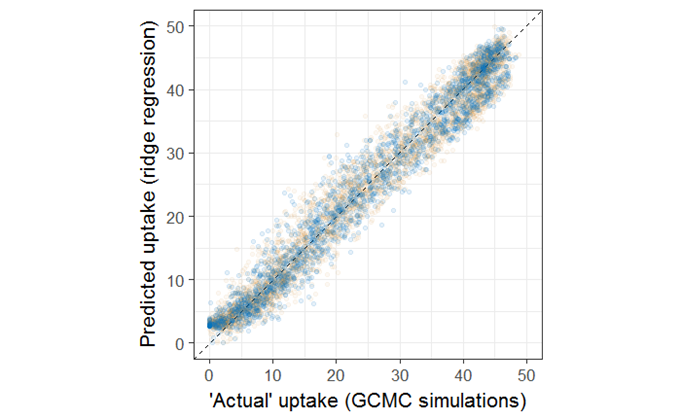
\includegraphics[width=0.75\columnwidth]{Figs/parity.png}
			\caption{Parity plot for (a) training and (b) test data on the energy histograms (TODO: split into two separate figures so it's more black and white-friendly, and easier to read without an animation)}
			\label{fig:parity}
		\end{figure}
		\2 Q2 of 0.96
		\2 RMSE of 3 g/L, MAE/MUE of 2.4 g/L
\end{outline}


\subsection{Screening}
\begin{outline}
	\1 Plan of testing applicability on 1000 MOFs
	\1 Benchmarking (maybe as a table): Full GCMC vs. energy grid calculations, feature representation, and ML
\end{outline}
\begin{figure}[!ht]
	\centering
	\caption{TODO: top candidates for experimental synthesis from the CCDC MOF database}
	\label{fig:candidates}
\end{figure}

\subsection{Generalizability to other gases}
\begin{outline}
	\1 See above
\end{outline}


\section{Acknowledgements}
Data Science Initiative, NMGC, etc.


\pagebreak
\section{Supporting Info}

\subsection{Hyperparameter tuning}

\begin{outline}
	\1 Grid spacing: convergence of a few different sample MOF histograms
		\2 Also might be good to have a figure overlaying sampling points on top of a continuous background, to exemplify the convergence testing
	\1 Bin width and degree of overlap (TODO: consider adding examples, and Q2 figure)
	\1 Lambda selection
	\begin{figure}[!ht]
		\centering
		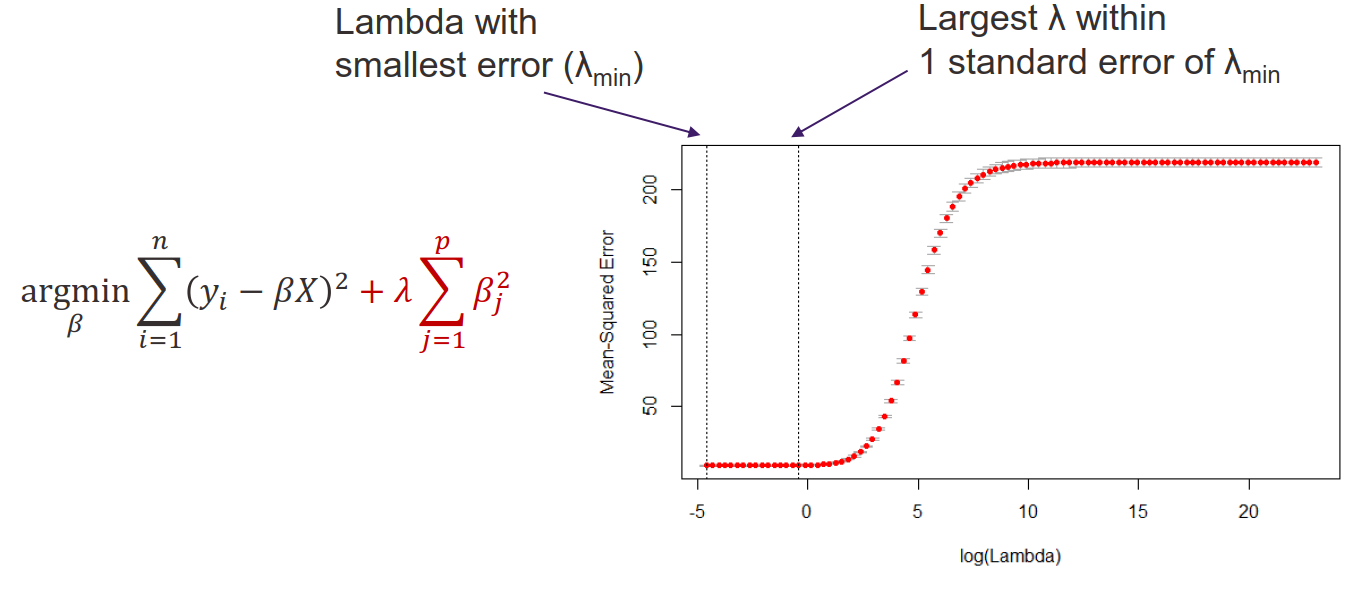
\includegraphics[width=0.75\columnwidth]{Figs/lambda.png}
		\caption{Determination of the regularization parameter $\lambda$ for ridge regression}
		\label{fig:lambda}
	\end{figure}
\end{outline}


\subsection{Model evaluation/consistency}

Also consider adding a figure on "Consistency across nodes/linkers and/or other DBs" (see Zr results)

\begin{figure}[!ht]
	\centering
	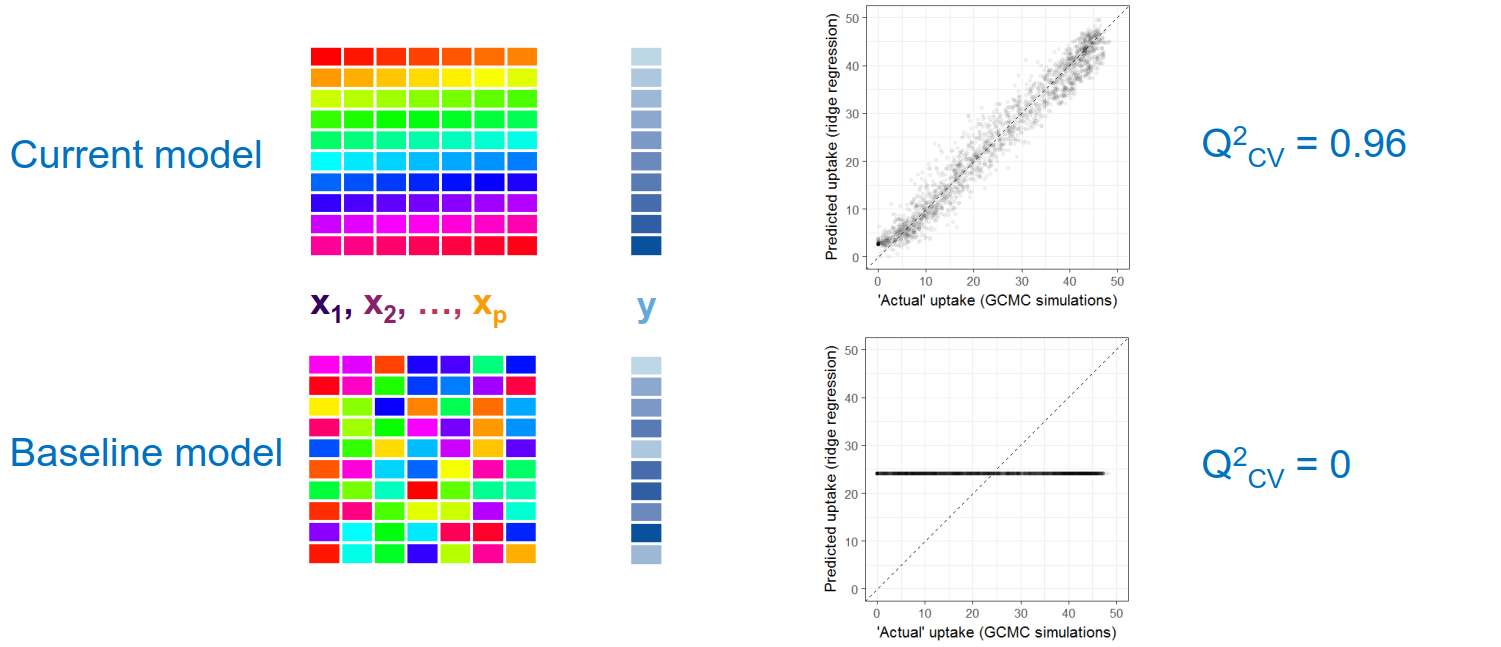
\includegraphics[width=0.75\columnwidth]{Figs/random_baseline.png}
	\caption{Comparison of $Q^2$ against a baseline of random data}
	\label{fig:q2_baseline}
\end{figure}

\begin{figure}[!ht]
	\centering
	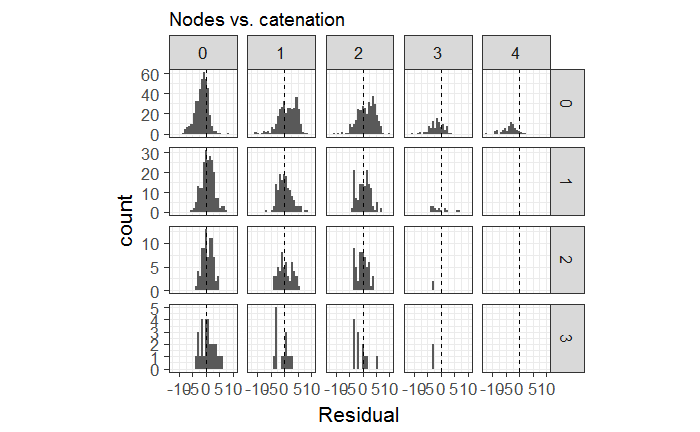
\includegraphics[width=0.75\columnwidth]{Figs/consistency_across_compositions.png}
	\caption{Consistency of model accuracy across MOF compositions.  Note that Zr MOFs are less accurate (node 4), possibly due to differences in topology and undersampling relative to \textbf{pcu} MOFs.}
	\label{fig:nodes_vs_cat}
\end{figure}

\subsection{Alternative approaches}

\begin{outline}
	\1 Benchmarking against traditional descriptors (textual properties like void fraction and density)
	\1 LASSO figure and coefficients
	\begin{figure}[!ht]
		\centering
		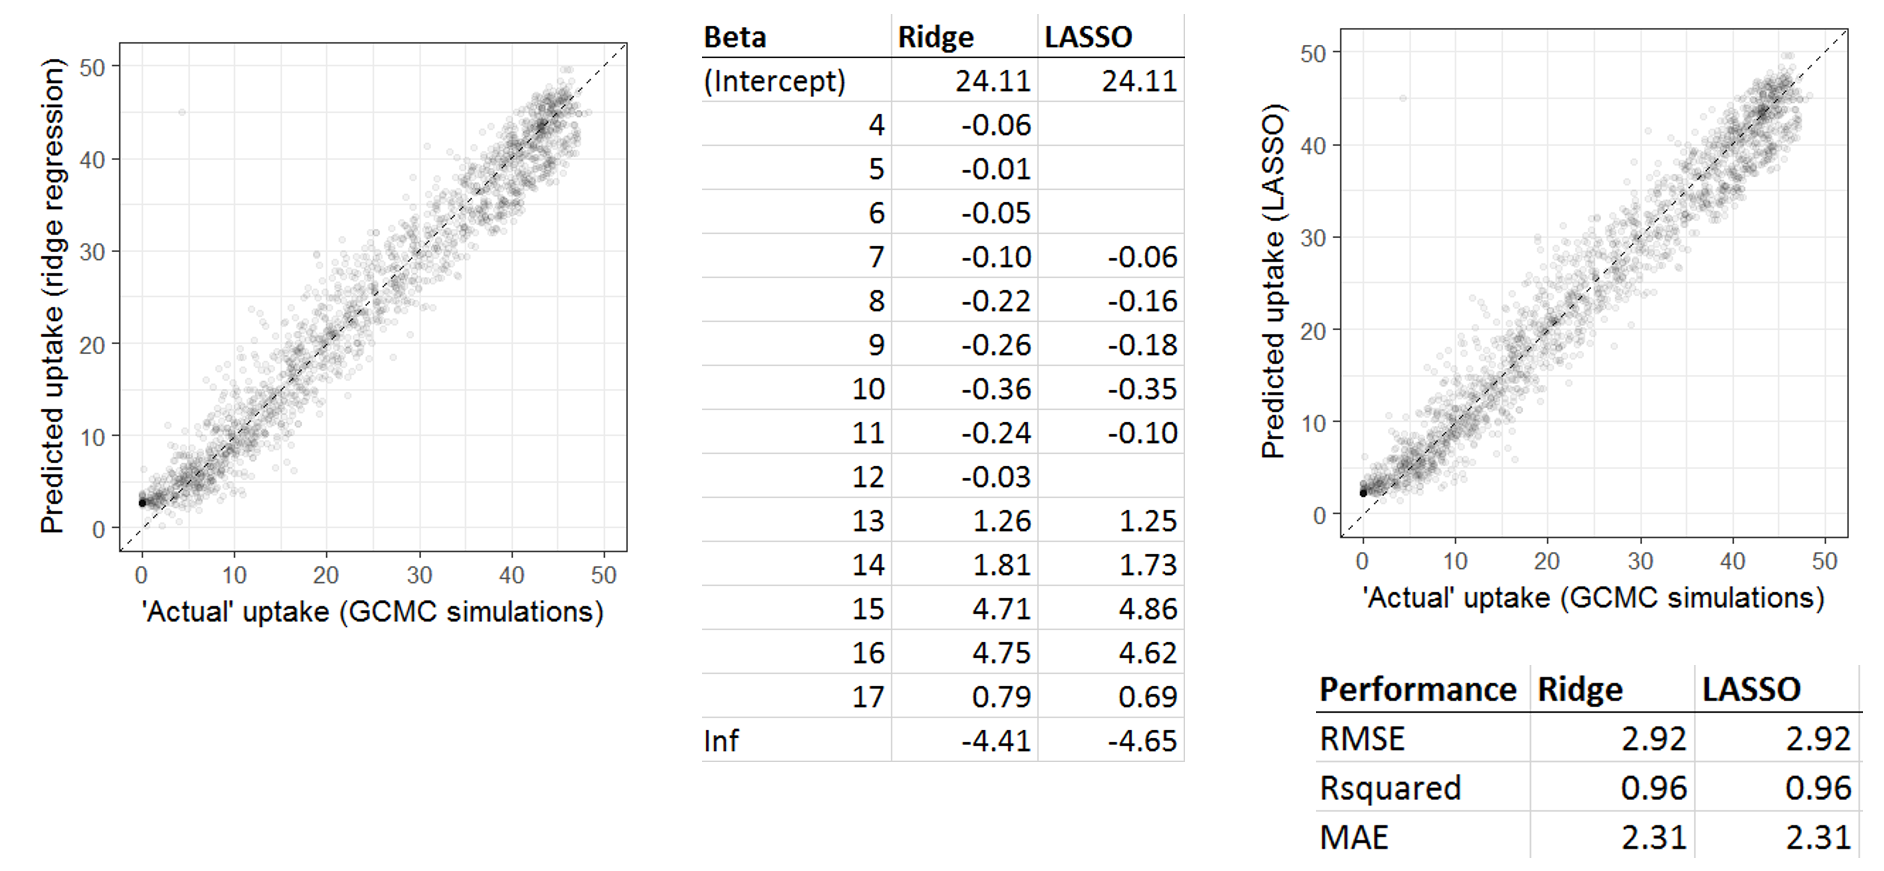
\includegraphics[width=0.75\columnwidth]{Figs/ridge_vs_lasso.png}
		\caption{Ridge regression and LASSO give similar results}
		\label{fig:lasso}
	\end{figure}
	
\end{outline}

\end{document}
